\section{Tracker Isolation Plots for all the $p_T$ bins}


In this note we will consider separate optimization of each isolation component individually, and
examine the effect of consecutive cuts.

Absolute isolation is shown in
Fig.~\ref{fig:PromptElecRecoPt_AbsIso} separately for each isolation variable as a function
of reconstructed $p_T$ for electrons and in Fig.... for muons. The`relative
isolation is shown in Fig.~\ref{fig:PromptElecRecoPt_RelIso} and Fig...., for electrons and
muons respectively.

 Particularly for soft electrons, the
 `explicit dependence of relative isolation on $p_T$ becomes apparent, while absolute isolation
 remains relatively constant across $p_T$ bins. Thus, for soft electrons we seek to optimize absolute
 isolation.

 \begin{figure}[htbp]
    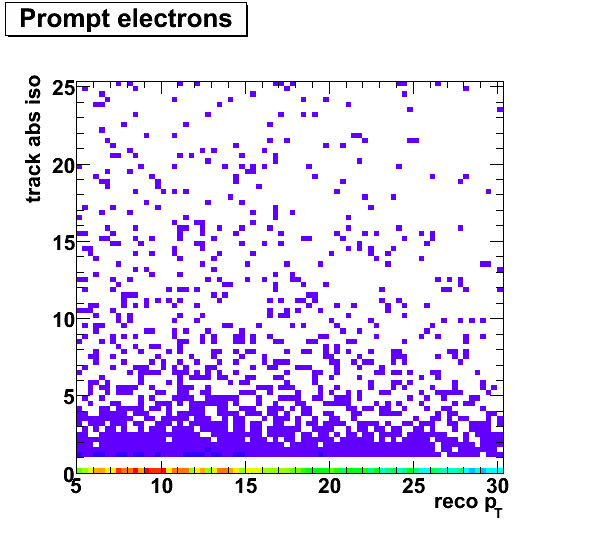
\includegraphics[width = 0.33\textwidth]{pictures/recoPt_absIso/trackIso_elec_prompt.png}
    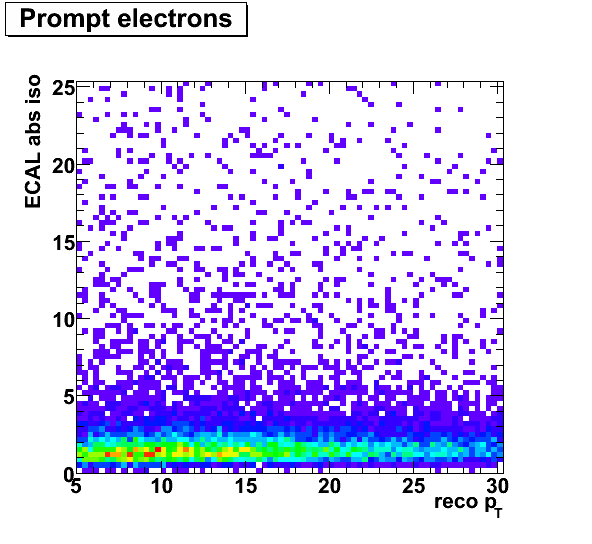
\includegraphics[width = 0.33\textwidth]{pictures/recoPt_absIso/ecalIso_elec_prompt.png}
    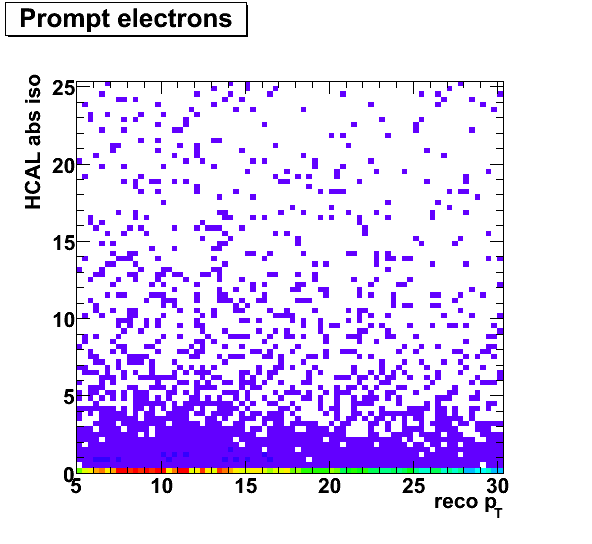
\includegraphics[width = 0.33\textwidth]{pictures/recoPt_absIso/hcalIso_elec_prompt.png}
    \caption{Absolute isolation calculated from (a) tracker, (b) ECAL and (c) HCAL as a function
       of reconstructed $p_{T}$ for prompt electrons}
    \label{fig:PromptElecRecoPt_AbsIso}
 \end{figure}

 \begin{figure}[htbp]
    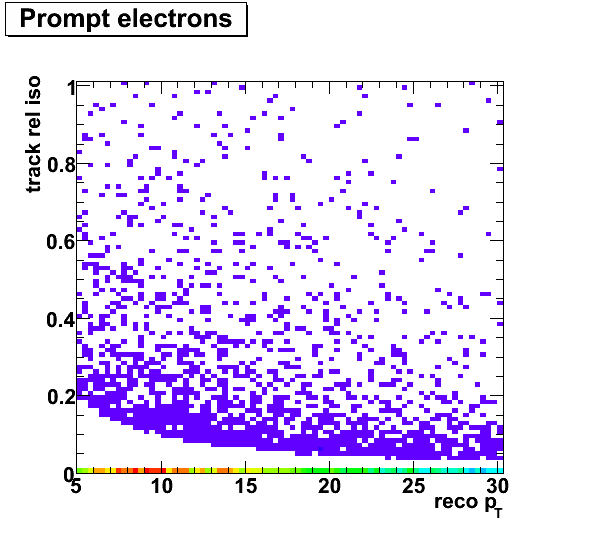
\includegraphics[width = 0.33\textwidth]{pictures/recoPt_relIso/trackIso_elec_prompt.png}
    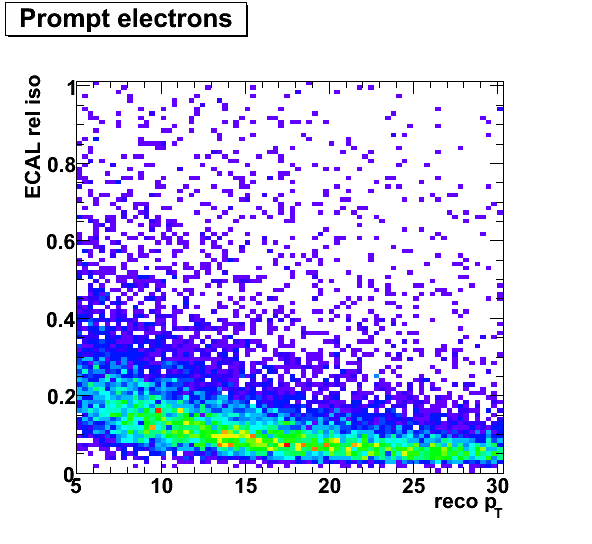
\includegraphics[width = 0.33\textwidth]{pictures/recoPt_relIso/ecalIso_elec_prompt.png}
    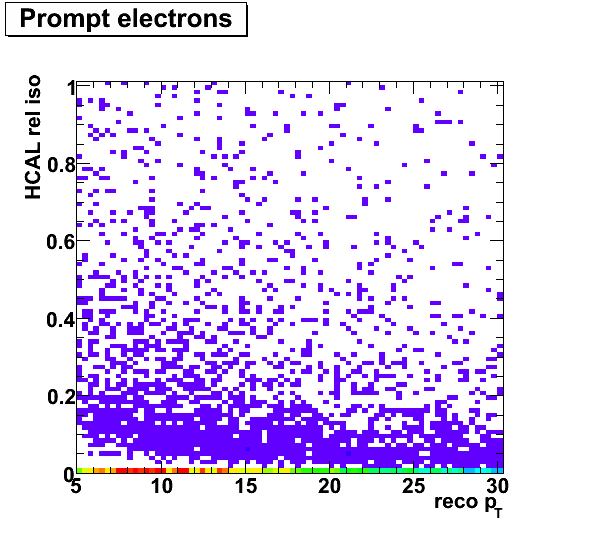
\includegraphics[width = 0.33\textwidth]{pictures/recoPt_relIso/hcalIso_elec_prompt.png}
    \caption{Relative isolation calculated from (a) tracker, (b) ECAL and (c) HCAL as a function of
       reconstructed $p_{T}$ for prompt electrons}
    \label{fig:PromptElecRecoPt_RelIso}
 \end{figure}

 \clearpage

 \begin{figure}[htbp]
    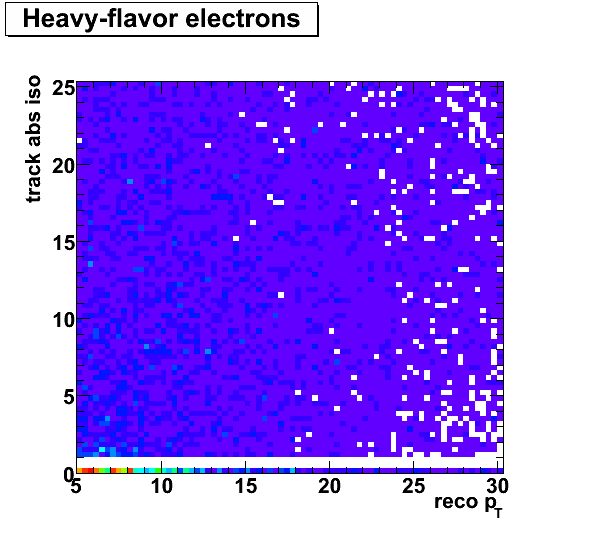
\includegraphics[width = 0.33\textwidth]{pictures/recoPt_absIso/trackIso_elec_nonPrompt.png}
    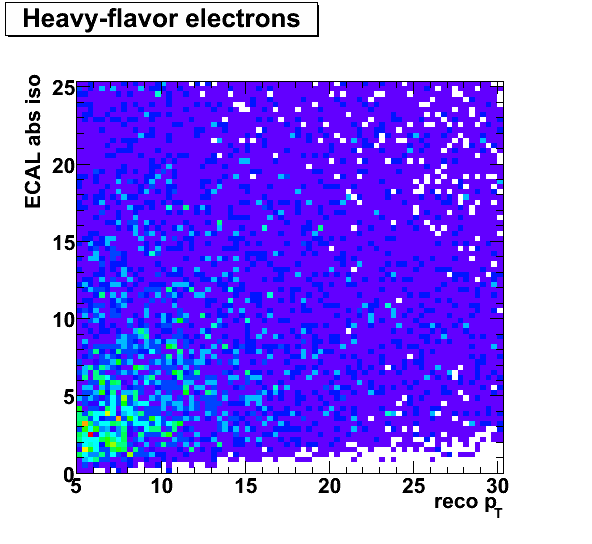
\includegraphics[width = 0.33\textwidth]{pictures/recoPt_absIso/ecalIso_elec_nonPrompt.png}
    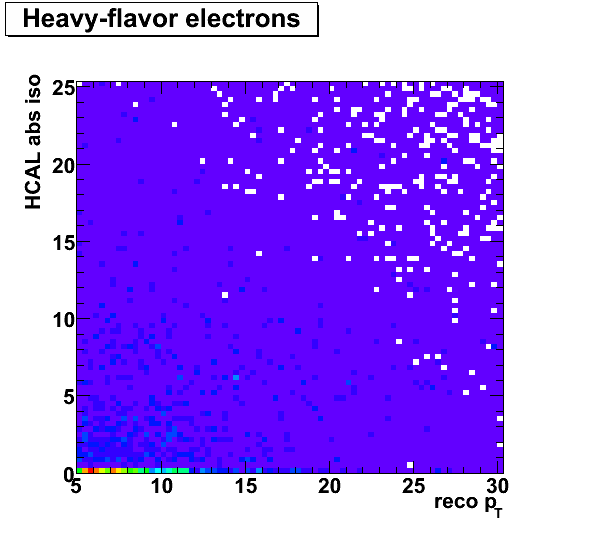
\includegraphics[width = 0.33\textwidth]{pictures/recoPt_absIso/hcalIso_elec_nonPrompt.png}
    \caption{Absolute isolation calculated from (a) tracker, (b) ECAL and (c) HCAL as a function of
       reconstructed $p_{T}$ for non-prompt electrons}
    \label{fig:NonPromptElecRecoPt_AbsIso}
 \end{figure}

 \begin{figure}[htbp]
    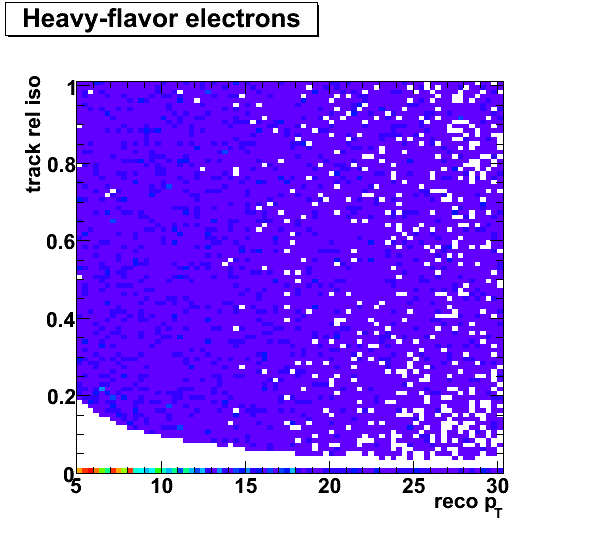
\includegraphics[width = 0.33\textwidth]{pictures/recoPt_relIso/trackIso_elec_nonPrompt.png}
    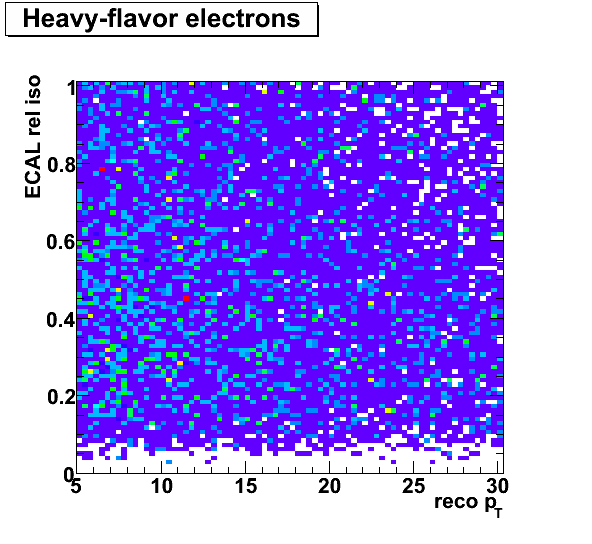
\includegraphics[width = 0.33\textwidth]{pictures/recoPt_relIso/ecalIso_elec_nonPrompt.png}
    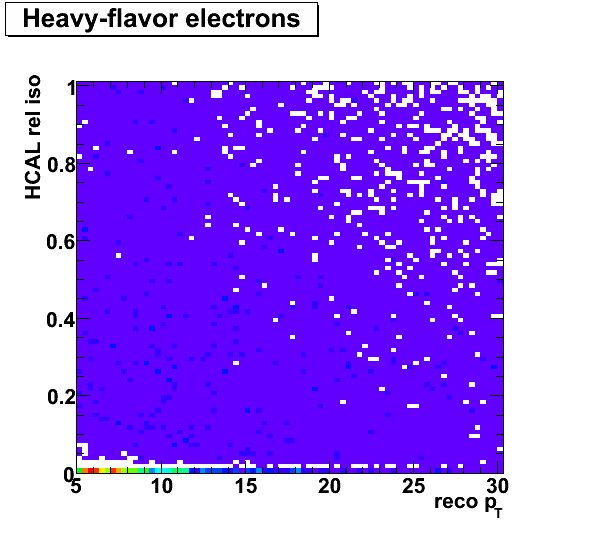
\includegraphics[width = 0.33\textwidth]{pictures/recoPt_relIso/hcalIso_elec_nonPrompt.png}
    \caption{Relative isolation calculated from (a) tracker, (b) ECAL and (c) HCAL as a function of
       reconstructed $p_{T}$ for non-prompt electrons}
    \label{fig:NonPromptElecRecoPt_RelIso}
 \end{figure}

 \clearpage

 \begin{figure}[htbp]
    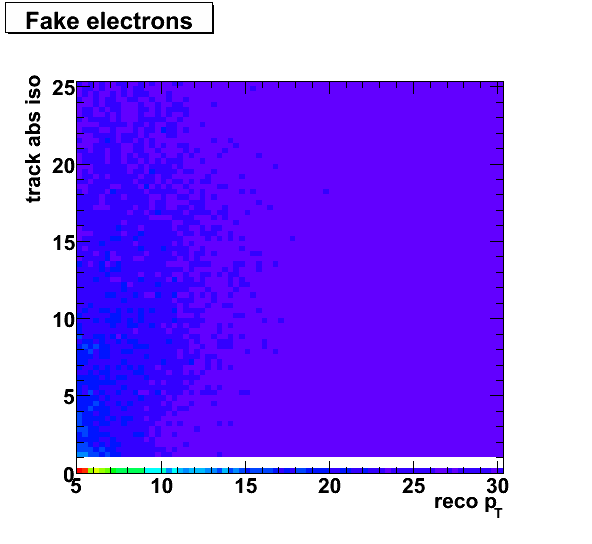
\includegraphics[width = 0.33\textwidth]{pictures/recoPt_absIso/trackIso_elec_fake.png}
    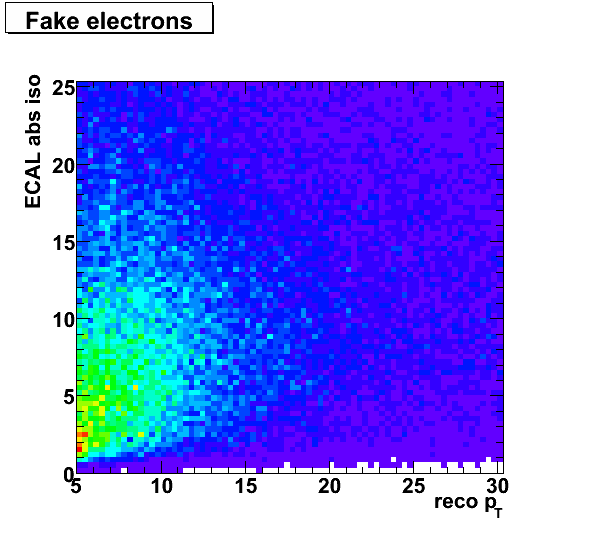
\includegraphics[width = 0.33\textwidth]{pictures/recoPt_absIso/ecalIso_elec_fake.png}
    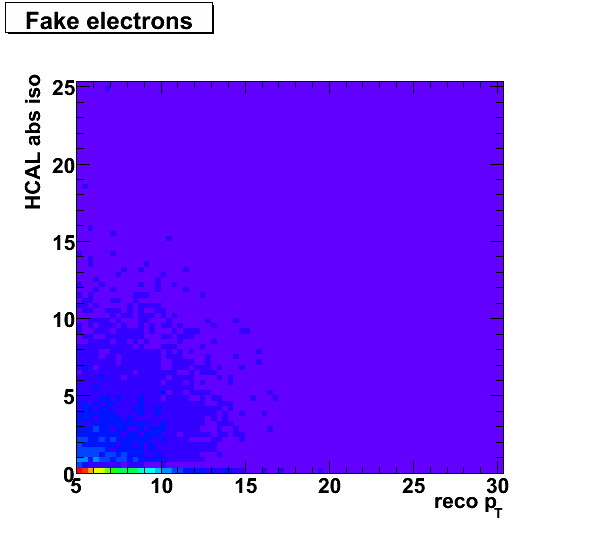
\includegraphics[width = 0.33\textwidth]{pictures/recoPt_absIso/hcalIso_elec_fake.png}
    \caption{Absolute isolation calculated from (a) tracker, (b) ECAL and (c) HCAL  as a function of
       reconstructed $p_{T}$ for fake electrons}
    \label{fig:FakeElecRecoPt_AbsIso}
 \end{figure}

 \begin{figure}[htbp]
    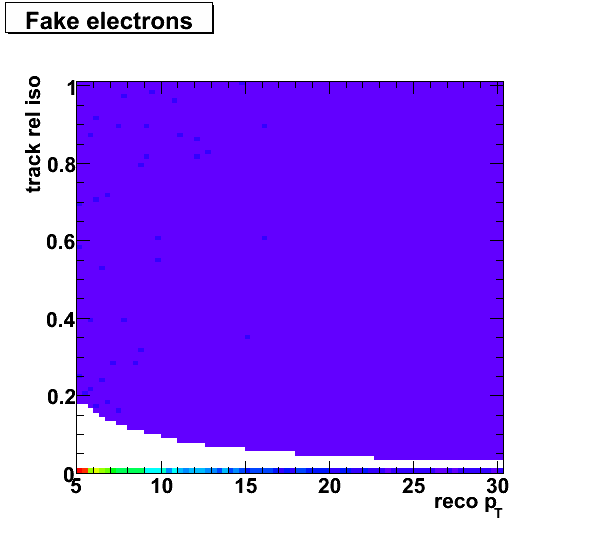
\includegraphics[width = 0.33\textwidth]{pictures/recoPt_relIso/trackIso_elec_fake.png}
    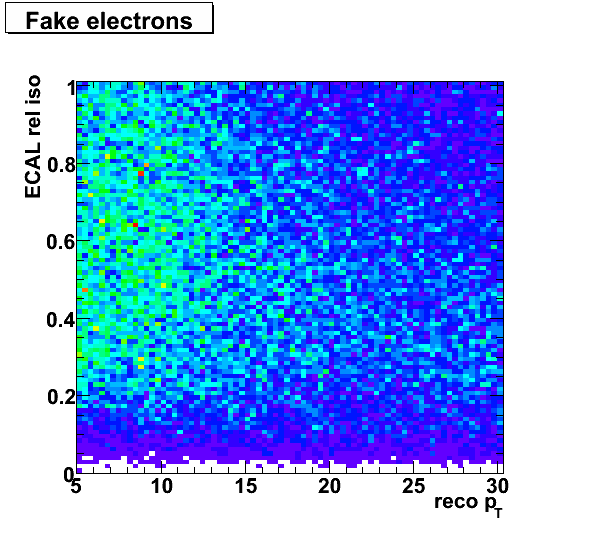
\includegraphics[width = 0.33\textwidth]{pictures/recoPt_relIso/ecalIso_elec_fake.png}
    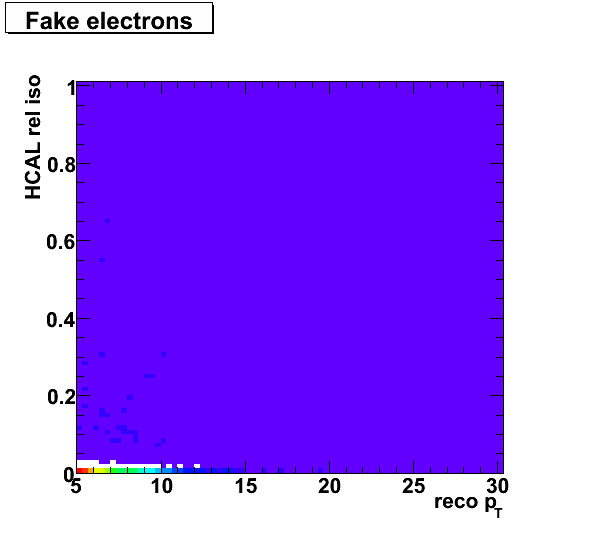
\includegraphics[width = 0.33\textwidth]{pictures/recoPt_relIso/hcalIso_elec_fake.png}
    \caption{Relative isolation calculated from (a) tracker, (b) ECAL and (c) HCAL as a function of
       reconstructed $p_{T}$ for fake electrons}
    \label{fig:FakeElecRecoPt_RelIso}
 \end{figure}

 \clearpage

 \begin{figure}[htbp]
    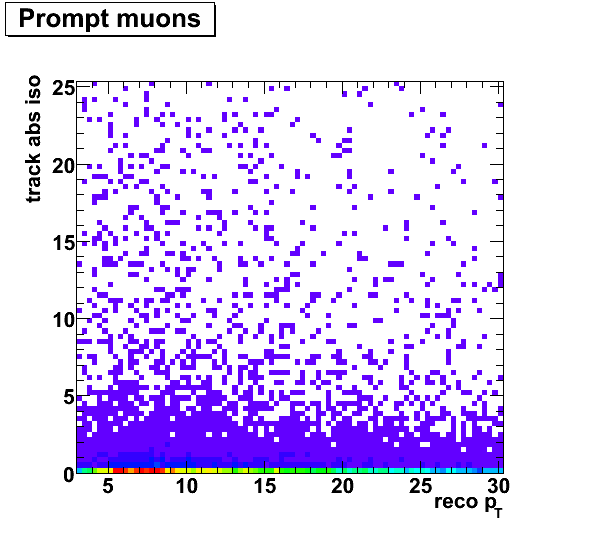
\includegraphics[width = 0.33\textwidth]{pictures/recoPt_absIso/trackIso_muon_prompt.png}
    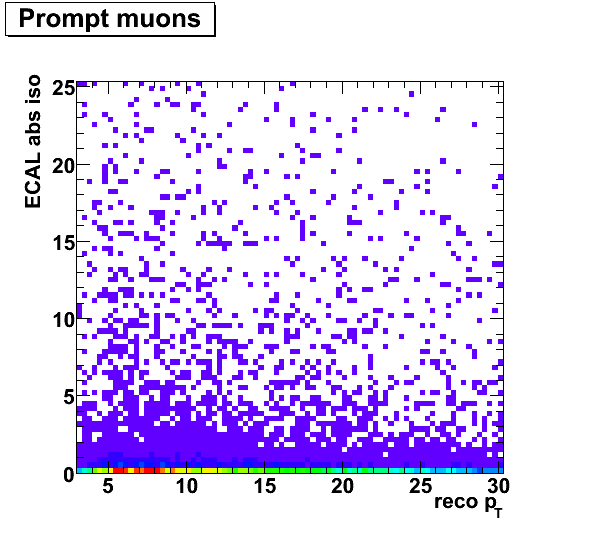
\includegraphics[width = 0.33\textwidth]{pictures/recoPt_absIso/ecalIso_muon_prompt.png}
    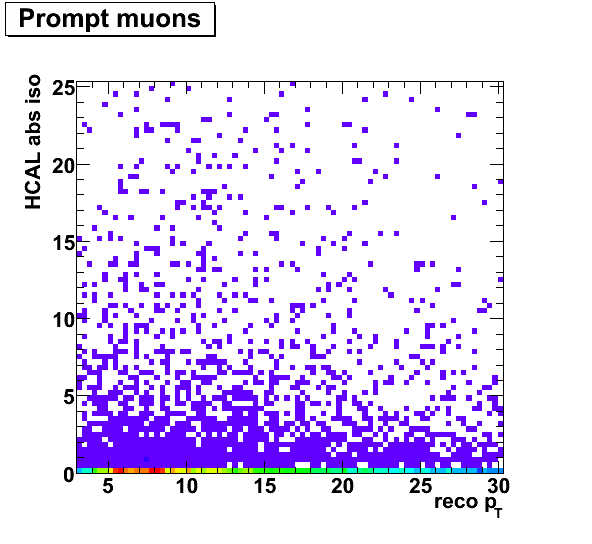
\includegraphics[width = 0.33\textwidth]{pictures/recoPt_absIso/hcalIso_muon_prompt.png}
    \caption{Absolute isolation calculated from (a) tracker, (b) ECAL and (c) HCAL versus
       reconstructed $p_{T}$ for prompt muons}
    \label{fig:PromptMuonRecoPt_AbsIso}
 \end{figure}

 \begin{figure}[htbp]
    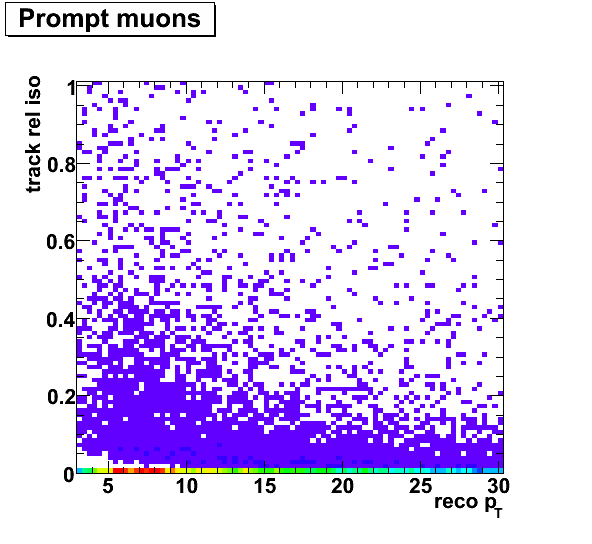
\includegraphics[width = 0.33\textwidth]{pictures/recoPt_relIso/trackIso_muon_prompt.png}
    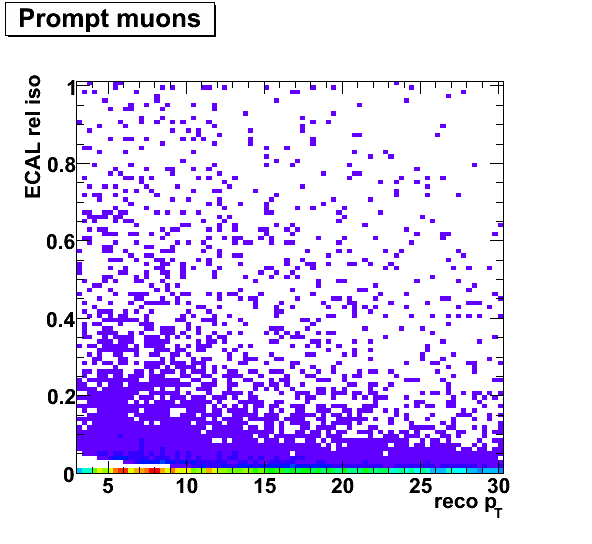
\includegraphics[width = 0.33\textwidth]{pictures/recoPt_relIso/ecalIso_muon_prompt.png}
    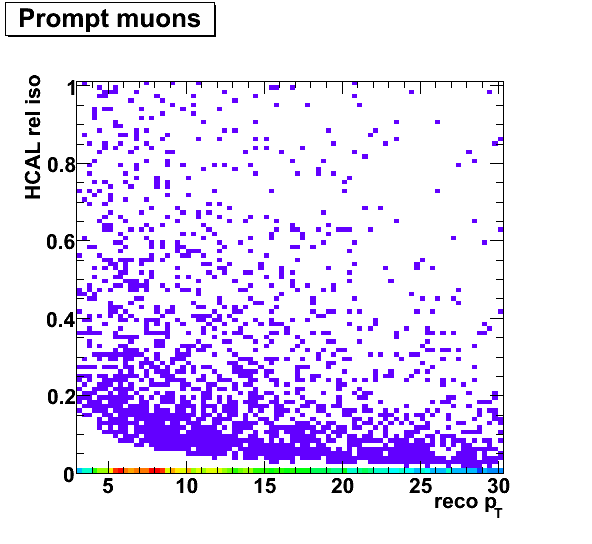
\includegraphics[width = 0.33\textwidth]{pictures/recoPt_relIso/hcalIso_muon_prompt.png}
    \caption{Relative isolation calculated from (a) tracker, (b) ECAL and (c) HCAL versus
       reconstructed $p_{T}$ for prompt muons}
    \label{fig:PromptMuonRecoPt_RelIso}
 \end{figure}

 \clearpage

 \begin{figure}[htbp]
    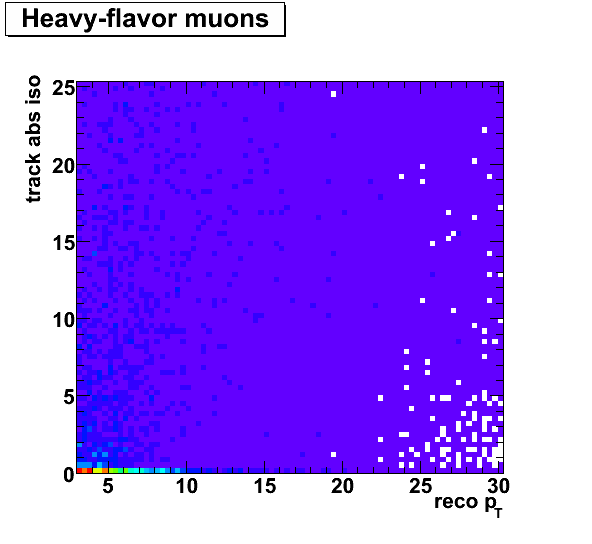
\includegraphics[width = 0.33\textwidth]{pictures/recoPt_absIso/trackIso_muon_nonPrompt.png}
    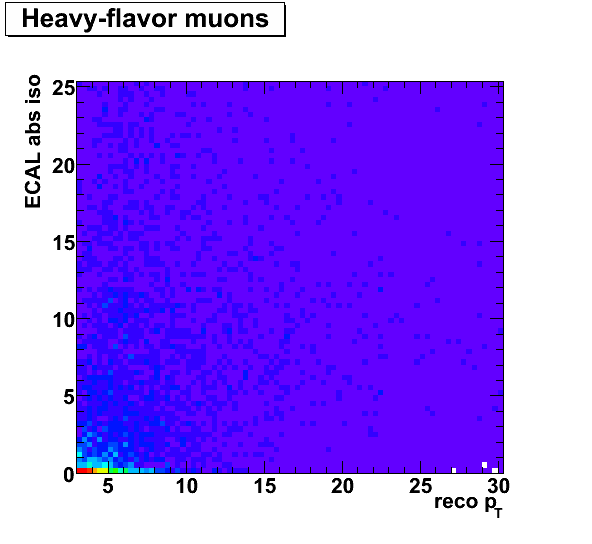
\includegraphics[width = 0.33\textwidth]{pictures/recoPt_absIso/ecalIso_muon_nonPrompt.png}
    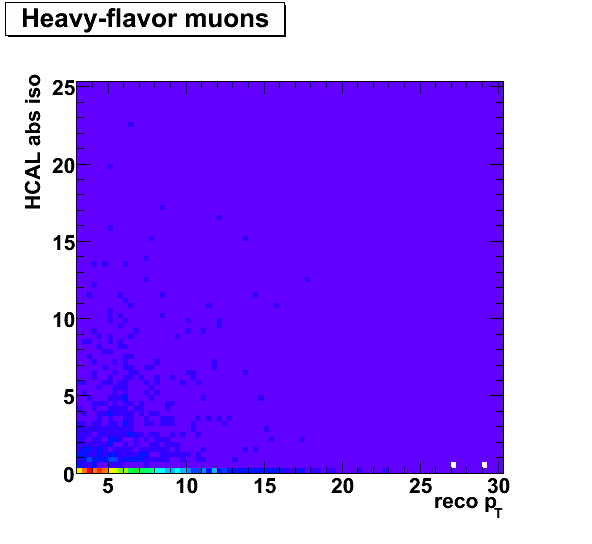
\includegraphics[width = 0.33\textwidth]{pictures/recoPt_absIso/hcalIso_muon_nonPrompt.png}
    \caption{Absolute isolation calculated from (a) tracker, (b) ECAL and (c) HCAL versus
       reconstructed $p_{T}$ for hadronic muons}
    \label{fig:NonPromptMuonRecoPt_AbsIso}
 \end{figure}

 \begin{figure}[htbp]
    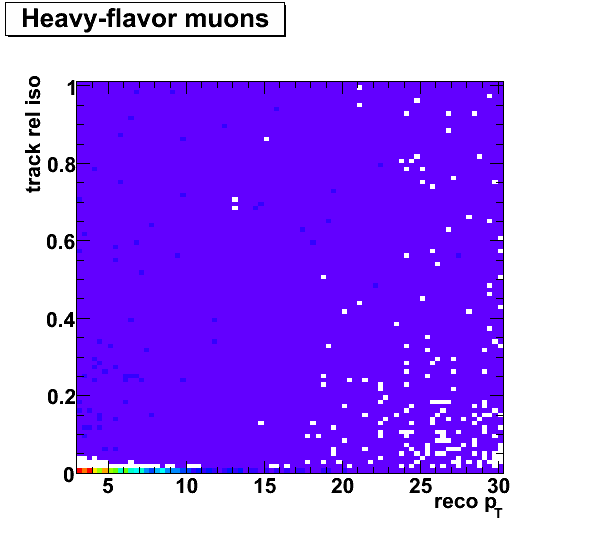
\includegraphics[width = 0.33\textwidth]{pictures/recoPt_relIso/trackIso_muon_nonPrompt.png}
    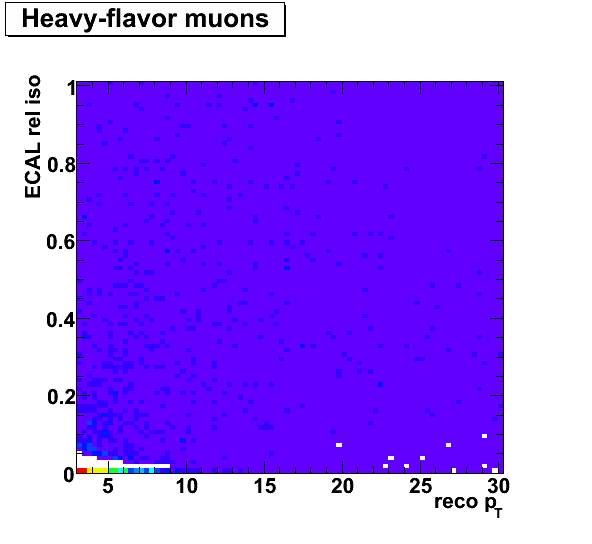
\includegraphics[width = 0.33\textwidth]{pictures/recoPt_relIso/ecalIso_muon_nonPrompt.png}
    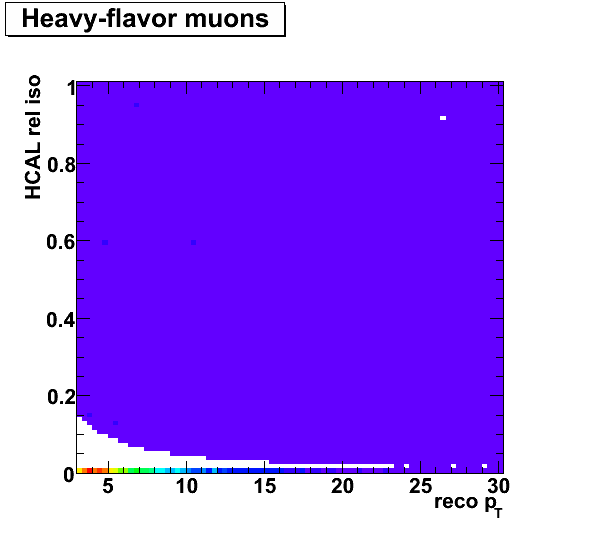
\includegraphics[width = 0.33\textwidth]{pictures/recoPt_relIso/hcalIso_muon_nonPrompt.png}
    \caption{Relative isolation calculated from (a) tracker, (b) ECAL and (c) HCAL versus
       reconstructed $p_{T}$ for hadronic muons}
    \label{fig:NonPromptMuonRecoPt_RelIso}
 \end{figure}

 \clearpage

 \begin{figure}[htbp]
    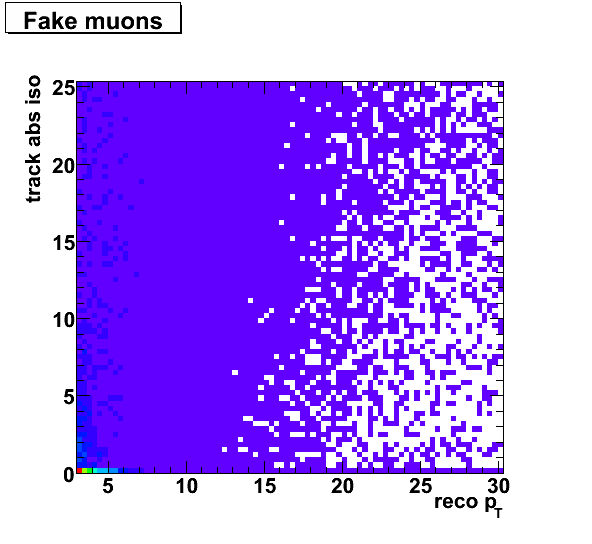
\includegraphics[width = 0.33\textwidth]{pictures/recoPt_absIso/trackIso_muon_fake.png}
   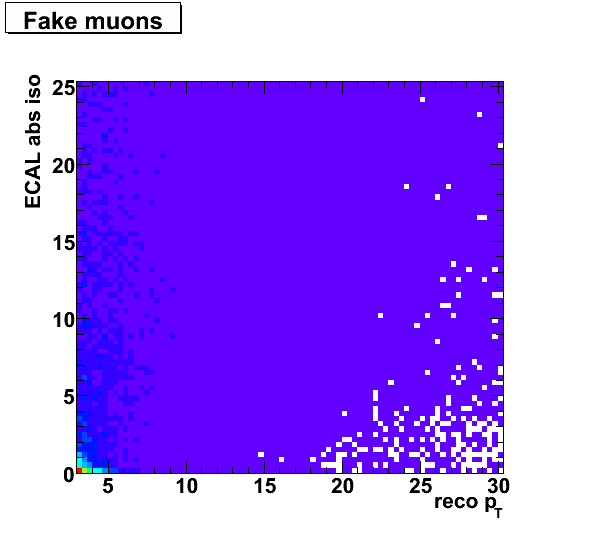
\includegraphics[width = 0.33\textwidth]{pictures/recoPt_absIso/ecalIso_muon_fake.png}
    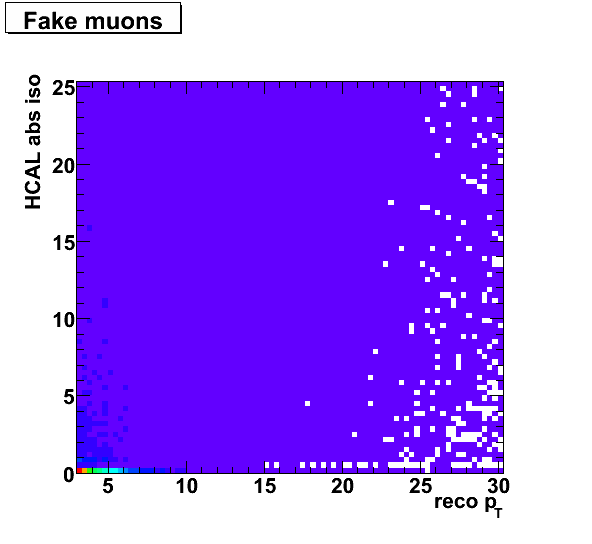
\includegraphics[width = 0.33\textwidth]{pictures/recoPt_absIso/hcalIso_muon_fake.png}
    \caption{Absolute isolation calculated from (a) tracker, (b) ECAL and (c) HCAL versus
       reconstructed $p_{T}$ for fake muons}
    \label{fig:FakeMuonRecoPt_AbsIso}
 \end{figure}

 \begin{figure}[htbp]
    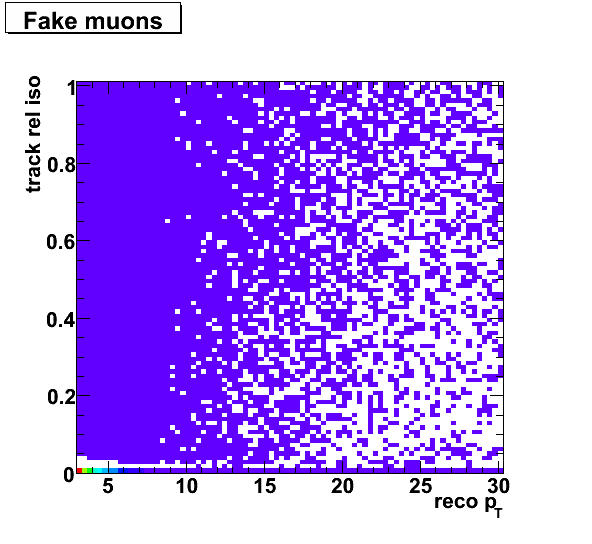
\includegraphics[width = 0.33\textwidth]{pictures/recoPt_relIso/trackIso_muon_fake.png}
    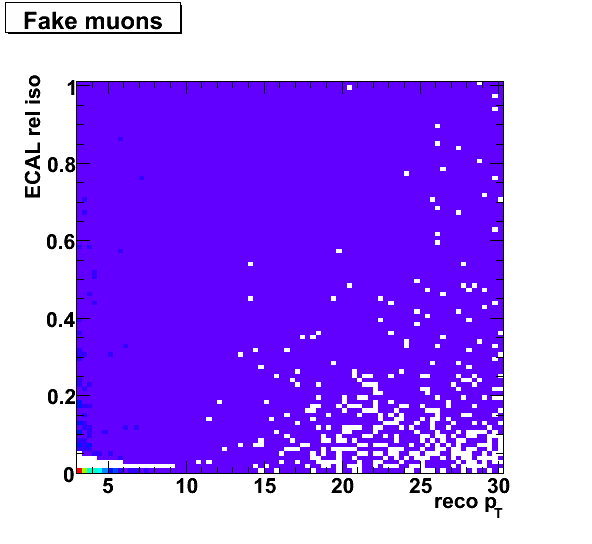
\includegraphics[width = 0.33\textwidth]{pictures/recoPt_relIso/ecalIso_muon_fake.png}
    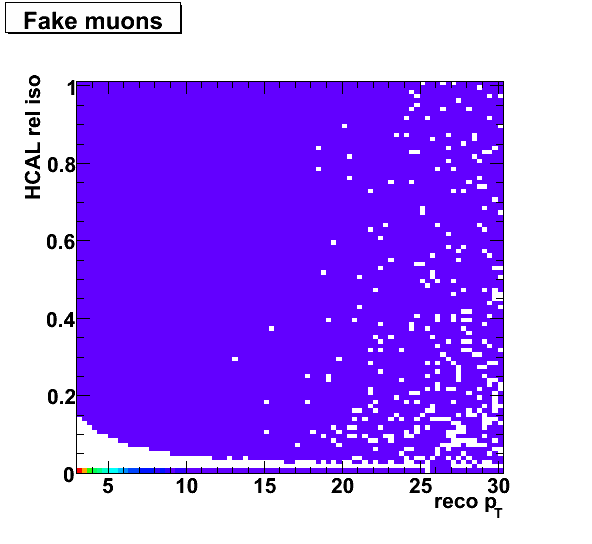
\includegraphics[width = 0.33\textwidth]{pictures/recoPt_relIso/hcalIso_muon_fake.png}
    \caption{Relative isolation calculated from (a) tracker, (b) ECAL and (c) HCAL versus
       reconstructed $p_{T}$ for fake muons}
    \label{fig:FakeMuonRecoPt_RelIso}
 \end{figure}

 \clearpage

 Figure~\ref{fig:AbsIsoCut_CutEffRej_Elec_PtCut0_PtCut1} shows the signal efficiency / background
 rejection of a cut on absolute isolation for electrons between 5 and 10 GeV.
 Figure~\ref{fig:AbsIsoCut_CutEffRej_Elec_PtCut4_PtCut5} shows these same curves for electrons
 between 25 and 30 GeV. We examine each $p_T$ range independently in order to optimize our isolation
 cut bin-by-bin.

 \begin{figure}[htbp]
    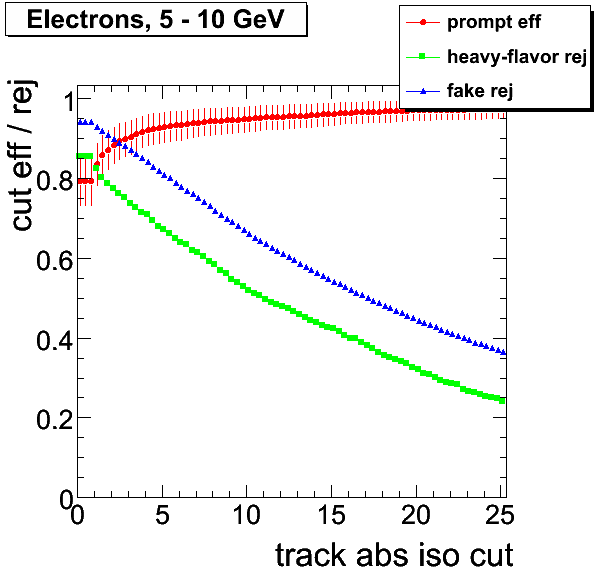
\includegraphics[width = 0.33\textwidth]{pictures/absIsoCut_absIsoCutEff/absIsoCut_trackIso_cutEff_elec_ptCut0_ptCut1.png}
    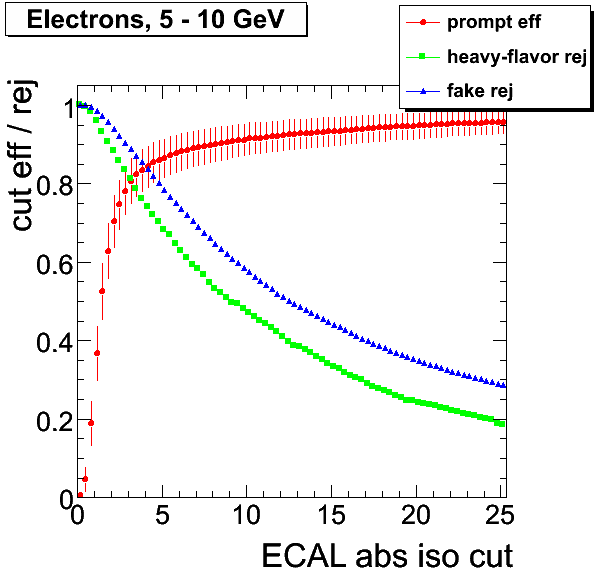
\includegraphics[width = 0.33\textwidth]{pictures/absIsoCut_absIsoCutEff/absIsoCut_ecalIso_cutEff_elec_ptCut0_ptCut1.png}
    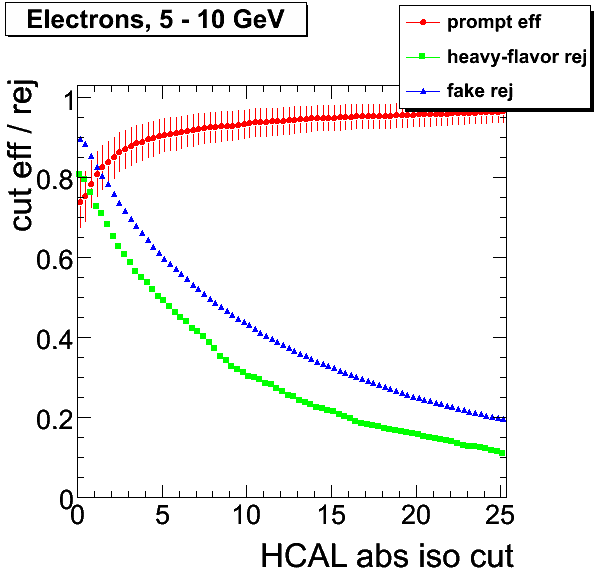
\includegraphics[width = 0.33\textwidth]{pictures/absIsoCut_absIsoCutEff/absIsoCut_hcalIso_cutEff_elec_ptCut0_ptCut1.png}
    \caption{Signal efficiency and background rejection ($1 -$ eff) of a cut on absolute isolation
       calculated from (a) the tracker, (b) the ECAL and (c) the HCAL for electrons with a
       reconstructed $p_{T}$ from 5 -- 10 GeV. The first curve indicates the efficiency for prompt
       electrons, the second curve indicates the rejection for hadronic electrons, and the third
       curve indicates the rejection for fake electrons.}
    \label{fig:AbsIsoCut_CutEffRej_Elec_PtCut0_PtCut1}
 \end{figure}

 \begin{figure}[htbp]
    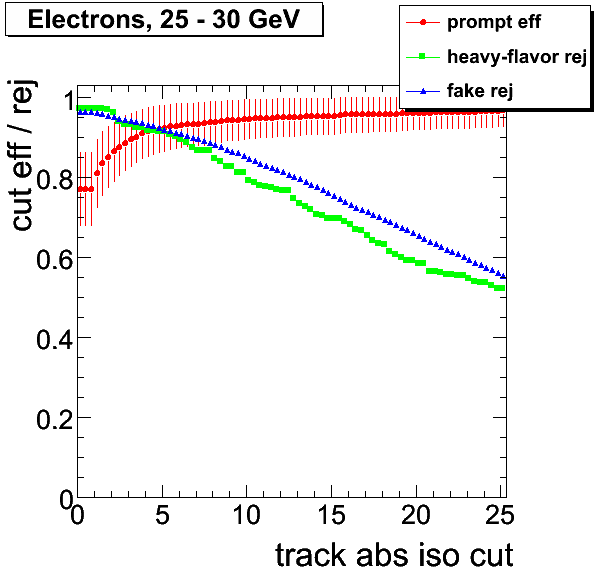
\includegraphics[width = 0.33\textwidth]{pictures/absIsoCut_absIsoCutEff/absIsoCut_trackIso_cutEff_elec_ptCut4_ptCut5.png}
    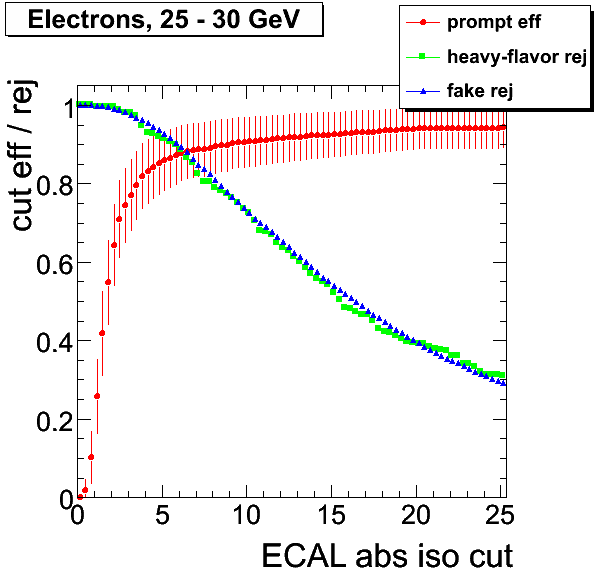
\includegraphics[width = 0.33\textwidth]{pictures/absIsoCut_absIsoCutEff/absIsoCut_ecalIso_cutEff_elec_ptCut4_ptCut5.png}
    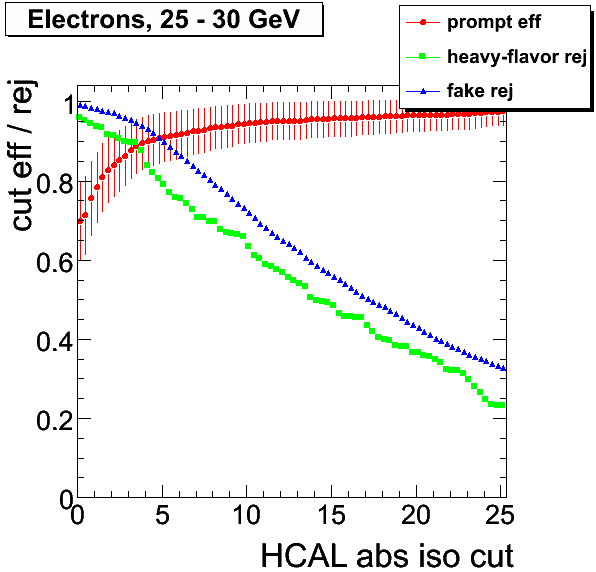
\includegraphics[width = 0.33\textwidth]{pictures/absIsoCut_absIsoCutEff/absIsoCut_hcalIso_cutEff_elec_ptCut4_ptCut5.png}
    \caption{Signal efficiency and background rejection ($1 -$ eff) of a cut on absolute isolation
       calculated from (a) the tracker, (b) the ECAL and (c) the HCAL for electrons with a
       reconstructed $p_{T}$ from 25 -- 30 GeV. The first curve indicates the efficiency for prompt
       electrons, the second curve indicates the rejection for hadronic electrons, and the third
       curve indicates the rejection for fake electrons.}
    \label{fig:AbsIsoCut_CutEffRej_Elec_PtCut4_PtCut5}
 \end{figure}

 \clearpage

 \begin{figure}[htbp]
    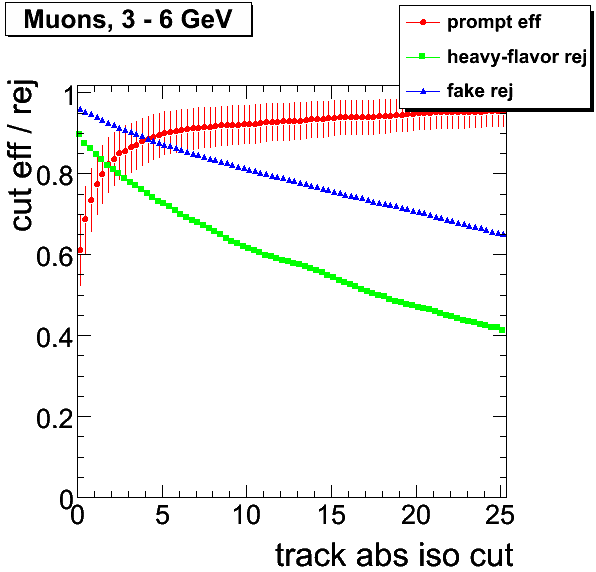
\includegraphics[width = 0.33\textwidth]{pictures/absIsoCut_absIsoCutEff/absIsoCut_trackIso_cutEff_muon_ptCut0_ptCut1.png}
    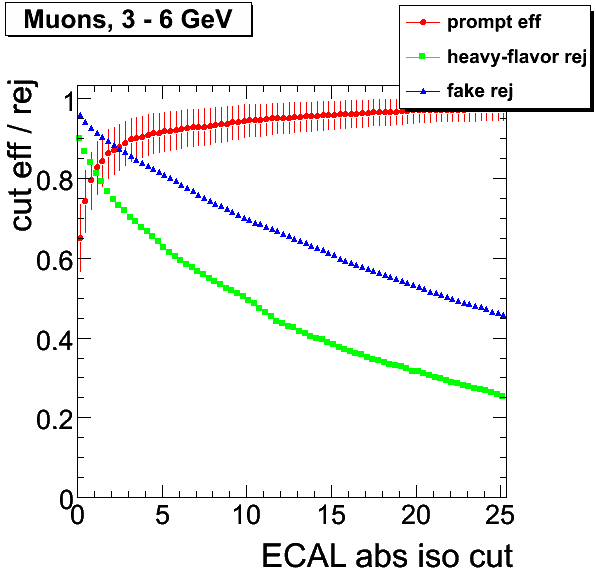
\includegraphics[width = 0.33\textwidth]{pictures/absIsoCut_absIsoCutEff/absIsoCut_ecalIso_cutEff_muon_ptCut0_ptCut1.png}
    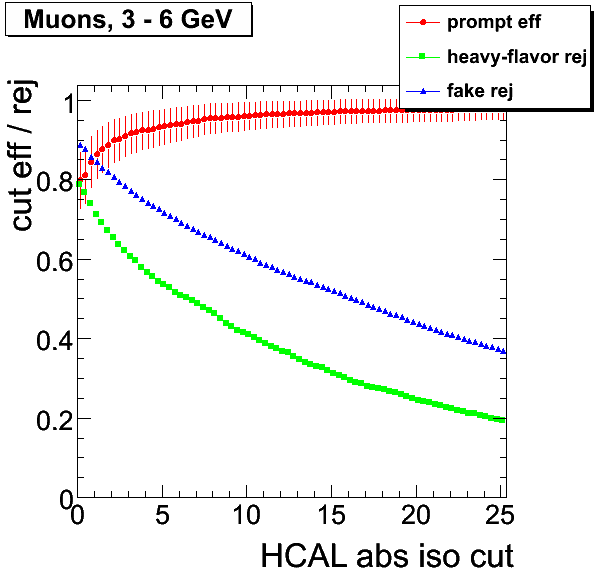
\includegraphics[width = 0.33\textwidth]{pictures/absIsoCut_absIsoCutEff/absIsoCut_hcalIso_cutEff_muon_ptCut0_ptCut1.png}
    \caption{Signal efficiency and background rejection ($1 - $ eff) of a cut on absolute isolation
       calculated from (a) the tracker, (b) the ECAL and (c) the HCAL for muons with a reconstructed
       $p_{T}$ from 3 -- 6 GeV. The first curve indicates the efficiency for prompt muons, the second
       curve indicates the rejection for hadronic muons, and the third curve indicates the rejection
       for fake muons.}
    \label{fig:AbsIsoCut_CutEffRej_Muon_PtCut0_PtCut1}
 \end{figure}

\begin{figure}[htbp]
   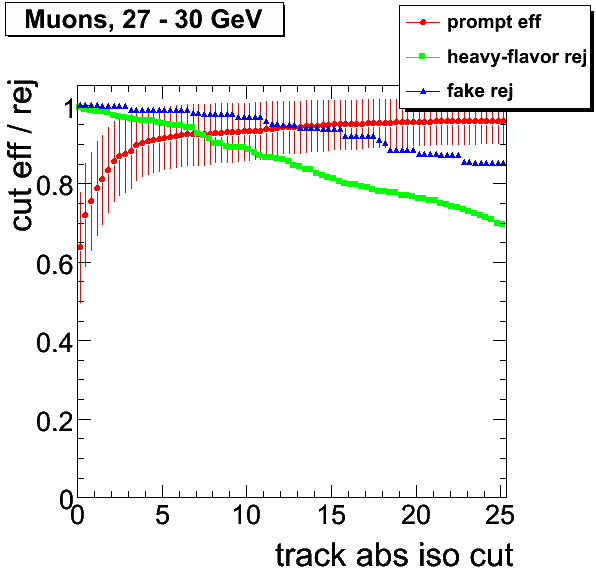
\includegraphics[width = 0.33\textwidth]{pictures/absIsoCut_absIsoCutEff/absIsoCut_trackIso_cutEff_muon_ptCut8_ptCut9.png}
   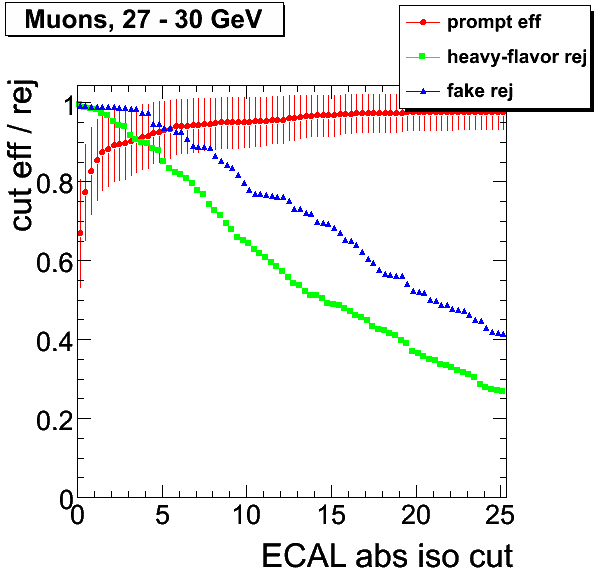
\includegraphics[width = 0.33\textwidth]{pictures/absIsoCut_absIsoCutEff/absIsoCut_ecalIso_cutEff_muon_ptCut8_ptCut9.png}
   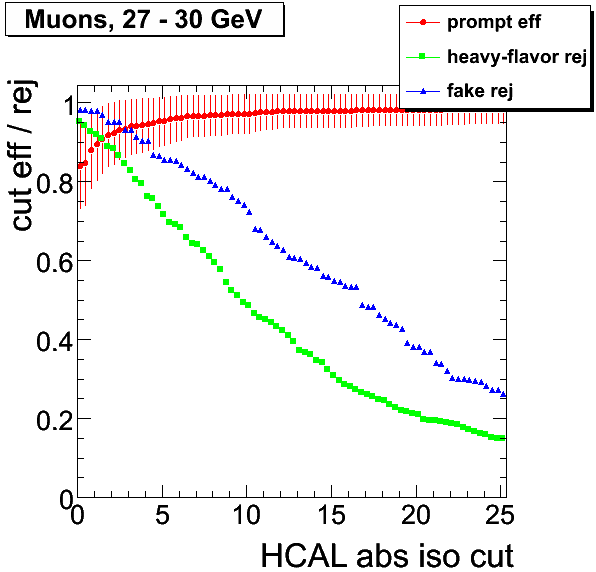
\includegraphics[width = 0.33\textwidth]{pictures/absIsoCut_absIsoCutEff/absIsoCut_hcalIso_cutEff_muon_ptCut8_ptCut9.png}
   \caption{Signal efficiency and background rejection ($1 - $ eff) of a cut on absolute isolation
      calculated from (a) the tracker, (b) the ECAL and (c) the HCAL for muons with a reconstructed
      $p_{T}$ from 15 -- 18 GeV. The first curve indicates the efficiency for prompt muons, the
      second curve indicates the rejection for hadronic muons, and the third curve indicates the
      rejection for fake muons.}
   \label{fig:AbsIsoCut_CutEffRej_Muon_PtCut4_PtCut5}
\end{figure}

\clearpage

\begin{figure}[htbp]
   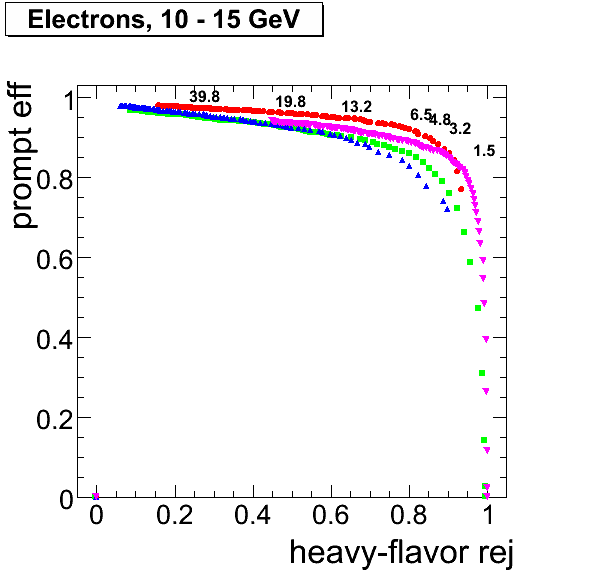
\includegraphics[width = 0.5\textwidth]{pictures/bkgdRej_sigEff/elec_nonPrompt_ptCut1_ptCut2.png}
   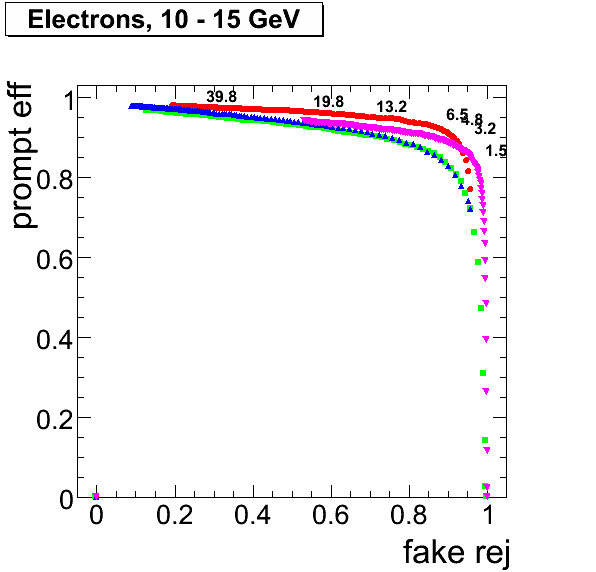
\includegraphics[width = 0.5\textwidth]{pictures/bkgdRej_sigEff/elec_fake_ptCut1_ptCut2.png}
   \caption{Electrons, 10 -- 15 GeV}
   \label{fig:elec_ptCut1_ptCut2}
\end{figure}

\begin{figure}[htbp]
   \includegraphics[width = 0.5\textwidth]{pictures/bkgdRej_sigEff/elec_nonPrompt_ptCut2_ptCut3.png}
   \includegraphics[width = 0.5\textwidth]{pictures/bkgdRej_sigEff/elec_fake_ptCut2_ptCut3.png}
   \caption{Electrons, 15 -- 20 GeV}
   \label{fig:elec_ptCut2_ptCut3}
\end{figure}

\begin{figure}[htbp]
   \includegraphics[width = 0.5\textwidth]{pictures/bkgdRej_sigEff/elec_nonPrompt_ptCut3_ptCut4.png}
   \includegraphics[width = 0.5\textwidth]{pictures/bkgdRej_sigEff/elec_fake_ptCut3_ptCut4.png}
   \caption{Electrons, 20 -- 25 GeV}
   \label{fig:elec_ptCut3_ptCut4}
\end{figure}

\begin{figure}[htbp]
   \includegraphics[width = 0.5\textwidth]{pictures/bkgdRej_sigEff/elec_nonPrompt_ptCut4_ptCut5.png}
   \includegraphics[width = 0.5\textwidth]{pictures/bkgdRej_sigEff/elec_fake_ptCut4_ptCut5.png}
   \caption{Electrons, 25 -- 30 GeV}
   \label{fig:elec_ptCut4_ptCut5}
\end{figure}

\clearpage

\begin{figure}[htbp]
   \includegraphics[width = 0.5\textwidth]{pictures/bkgdRej_sigEff/muon_nonPrompt_ptCut1_ptCut2.png}
   \includegraphics[width = 0.5\textwidth]{pictures/bkgdRej_sigEff/muon_fake_ptCut1_ptCut2.png}
   \caption{Muons, 6 -- 9 GeV}
   \label{fig:muon_ptCut1_ptCut2}
\end{figure}

\begin{figure}[htbp]
   \includegraphics[width = 0.5\textwidth]{pictures/bkgdRej_sigEff/muon_nonPrompt_ptCut2_ptCut3.png}
   \includegraphics[width = 0.5\textwidth]{pictures/bkgdRej_sigEff/muon_fake_ptCut2_ptCut3.png}
   \caption{Muons, 9 -- 12 GeV}
   \label{fig:muon_ptCut2_ptCut3}
\end{figure}

\begin{figure}[htbp]
   \includegraphics[width = 0.5\textwidth]{pictures/bkgdRej_sigEff/muon_nonPrompt_ptCut3_ptCut4.png}
   \includegraphics[width = 0.5\textwidth]{pictures/bkgdRej_sigEff/muon_fake_ptCut3_ptCut4.png}
   \caption{Muons, 12 -- 15 GeV}
   \label{fig:muon_ptCut3_ptCut4}
\end{figure}

\begin{figure}[htbp]
   \includegraphics[width = 0.5\textwidth]{pictures/bkgdRej_sigEff/muon_nonPrompt_ptCut4_ptCut5.png}
   \includegraphics[width = 0.5\textwidth]{pictures/bkgdRej_sigEff/muon_fake_ptCut4_ptCut5.png}
   \caption{Muons, 15 -- 18 GeV}
   \label{fig:muon_ptCut4_ptCut5}
\end{figure}

\clearpage

\begin{figure}[htbp]
   \includegraphics[width = 0.5\textwidth]{pictures/bkgdRej_sigEff/muon_nonPrompt_ptCut5_ptCut6.png}
   \includegraphics[width = 0.5\textwidth]{pictures/bkgdRej_sigEff/muon_fake_ptCut5_ptCut6.png}
   \caption{Muons, 18 -- 21 GeV}
   \label{fig:muon_ptCut5_ptCut6}
\end{figure}

\begin{figure}[htbp]
   \includegraphics[width = 0.5\textwidth]{pictures/bkgdRej_sigEff/muon_nonPrompt_ptCut6_ptCut7.png}
   \includegraphics[width = 0.5\textwidth]{pictures/bkgdRej_sigEff/muon_fake_ptCut6_ptCut7.png}
   \caption{Muons, 21 -- 24 GeV}
   \label{fig:muon_ptCut6_ptCut7}
\end{figure}

\begin{figure}[htbp]
   \includegraphics[width = 0.5\textwidth]{pictures/bkgdRej_sigEff/muon_nonPrompt_ptCut7_ptCut8.png}
   \includegraphics[width = 0.5\textwidth]{pictures/bkgdRej_sigEff/muon_fake_ptCut7_ptCut8.png}
   \caption{Muons, 24 -- 27 GeV}
   \label{fig:muon_ptCut7_ptCut8}
\end{figure}

\begin{figure}[htbp]
   \includegraphics[width = 0.5\textwidth]{pictures/bkgdRej_sigEff/muon_nonPrompt_ptCut8_ptCut9.png}
   \includegraphics[width = 0.5\textwidth]{pictures/bkgdRej_sigEff/muon_fake_ptCut8_ptCut9.png}
   \caption{Muons, 27 -- 30 GeV}
   \label{fig:muon_ptCut8_ptCut9}
\end{figure}

\clearpage

\begin{figure}[htbp]
   \includegraphics[width = 0.33\textwidth]{pictures/optIsoCut/trackIso_elec_pure.png}
   \includegraphics[width = 0.33\textwidth]{pictures/optIsoCut/trackIso_elec_opt.png}
   \includegraphics[width = 0.33\textwidth]{pictures/optIsoCut/trackIso_elec_eff.png}
   \label{fig:optTrackIso_elec}
\end{figure}

\begin{figure}[htbp]
   \includegraphics[width = 0.33\textwidth]{pictures/optIsoCut/trackIso_muon_pure.png}
   \includegraphics[width = 0.33\textwidth]{pictures/optIsoCut/trackIso_muon_opt.png}
   \includegraphics[width = 0.33\textwidth]{pictures/optIsoCut/trackIso_muon_eff.png}
   \label{fig:optTrackIso_muon}
\end{figure}

\begin{figure}[htbp]
   \includegraphics[width = 0.33\textwidth]{pictures/optIsoCut/ecalIso_elec_pure.png}
   \includegraphics[width = 0.33\textwidth]{pictures/optIsoCut/ecalIso_elec_opt.png}
   \includegraphics[width = 0.33\textwidth]{pictures/optIsoCut/ecalIso_elec_eff.png}
   \label{fig:optEcalIso_elec}
\end{figure}

\begin{figure}[htbp]
   \includegraphics[width = 0.33\textwidth]{pictures/optIsoCut/ecalIso_muon_pure.png}
   \includegraphics[width = 0.33\textwidth]{pictures/optIsoCut/ecalIso_muon_opt.png}
   \includegraphics[width = 0.33\textwidth]{pictures/optIsoCut/ecalIso_muon_eff.png}
   \label{fig:optEcalIso_muon}
\end{figure}

\begin{figure}[htbp]
   \includegraphics[width = 0.33\textwidth]{pictures/optIsoCut/hcalIso_elec_pure.png}
   \includegraphics[width = 0.33\textwidth]{pictures/optIsoCut/hcalIso_elec_opt.png}
   \includegraphics[width = 0.33\textwidth]{pictures/optIsoCut/hcalIso_elec_eff.png}
   \label{fig:optHcalIso_elec}
\end{figure}

\begin{figure}[htbp]
   \includegraphics[width = 0.33\textwidth]{pictures/optIsoCut/hcalIso_muon_pure.png}
   \includegraphics[width = 0.33\textwidth]{pictures/optIsoCut/hcalIso_muon_opt.png}
   \includegraphics[width = 0.33\textwidth]{pictures/optIsoCut/hcalIso_muon_eff.png}
   \label{fig:optHcalIso_muon}
\end{figure}
